\chapter{Knee Joint Design}

% The knee joint presented in this thesis is designed to replace the current passive pin knee joint with a spring wrap clutch for the WPI LARRE exoskeleton (see \autoref{sec:larre}).

% \TODO{add more in the intro section for the knee joint design}

\section{Design Requirements}
\label{sec:DesignParams}
The following are the design parameters layed out at the beginning of the project:

\subsubsection{Follows the defined knee tibiofemoral trajectory}
The knee joint must be able to follow a tibiofemoral trajectory. As referenced in \cite{KinDynKneeJoint}, human knee joints can be generally defined by a quartic trajectory. This project will use the parameters of a cadaver, which can be seen in \autoref{eq:KneeJointGeometryEquation}. The design of the joint must be easily customizable for each patient/user. Ideally, all parts except a few should remain the same to increase simplicity and reduce cost of manufacturing.

\begin{equation}
    r(\theta) mm = 1.078\theta^4 - 11.184\theta^3 + 26.524\theta^2 - 0.825\theta + 263.59
    \label{eq:KneeJointGeometryEquation}
\end{equation}

\subsubsection{Supports the weight of a person}
Each joint should be able to support half of the weight of a 85kg human plus a 15kg exoskeleton (total of 100kg) with an additional safety factor. 

\subsubsection{Power/Torqe/Speed for walking gaits and sit/stand exercises}

\begin{figure}[ht!]
    \centering
    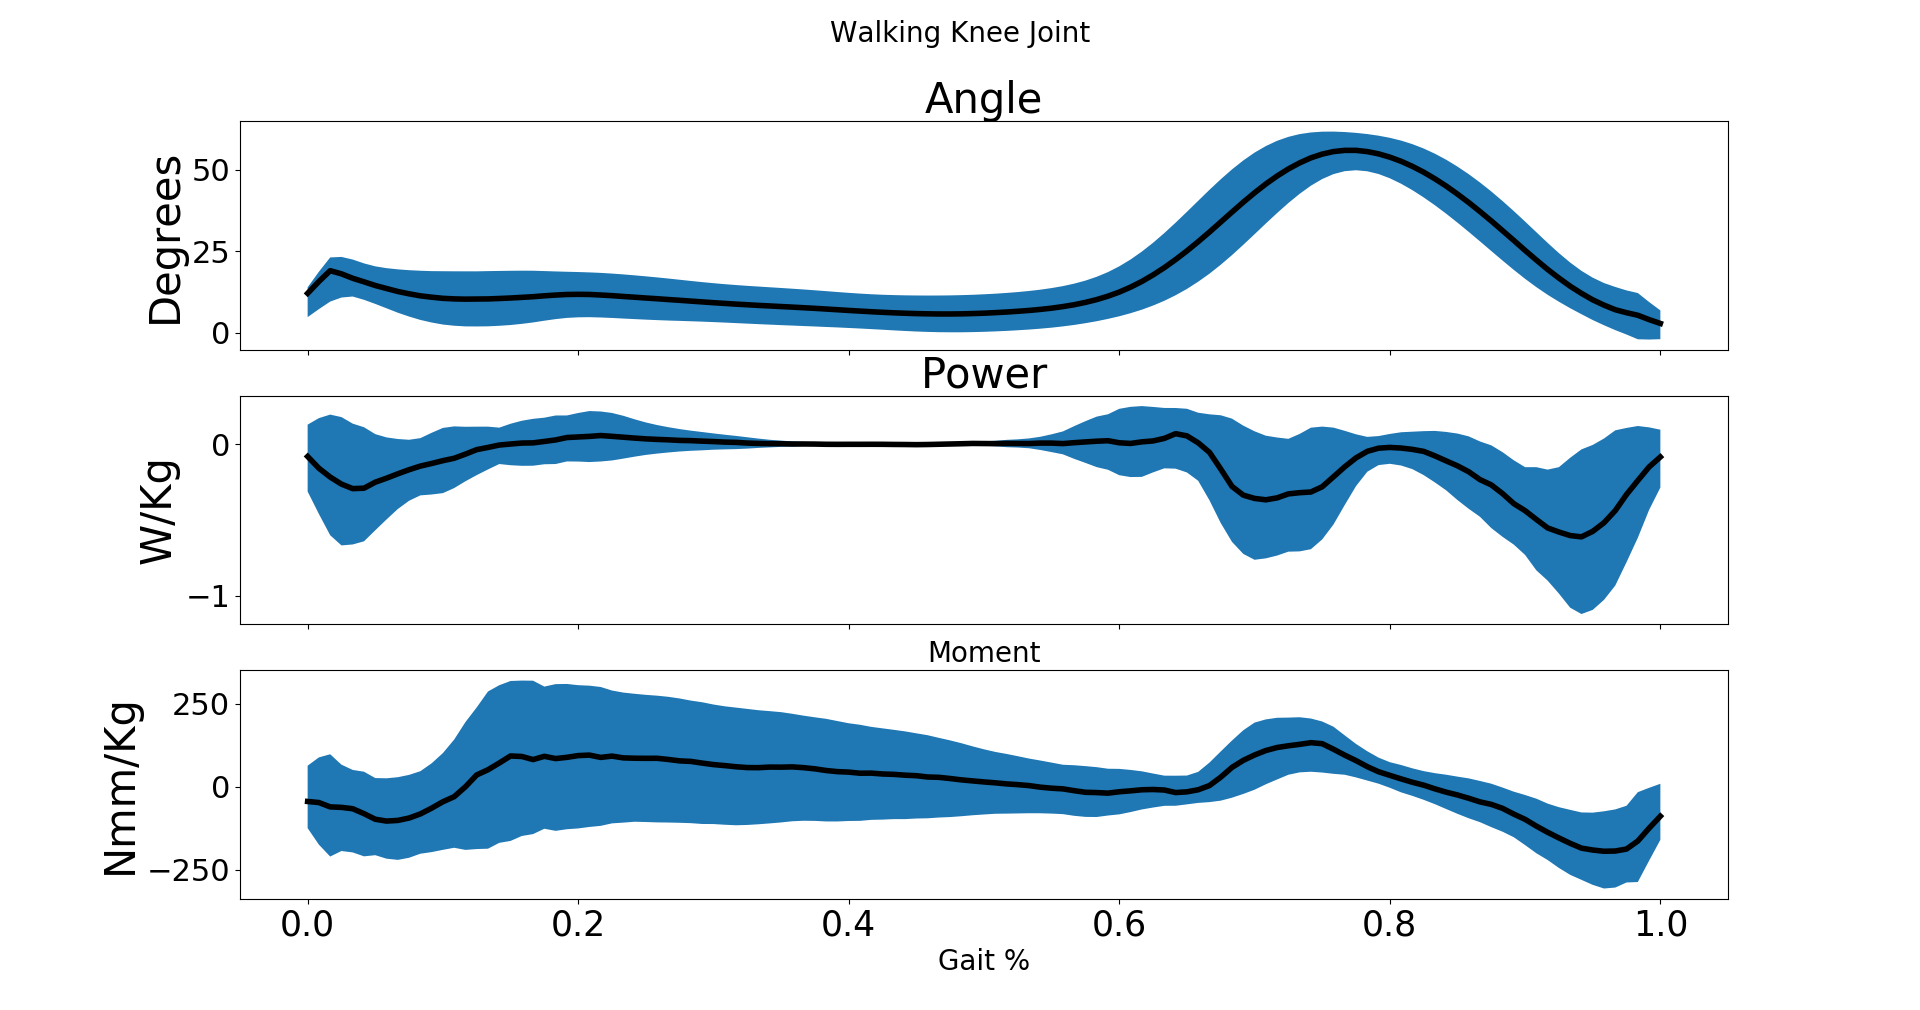
\includegraphics[width=\linewidth]{Figures/Design/WalkingPowerCurveKnee.png}
    \caption{Joint kinematics and dynamics during a walking gait cycle \cite{SpringWrapClutchKnee}}
    \label{fig:WalkingPowerCurve}
\end{figure}

\begin{figure}[ht!]
    \centering
    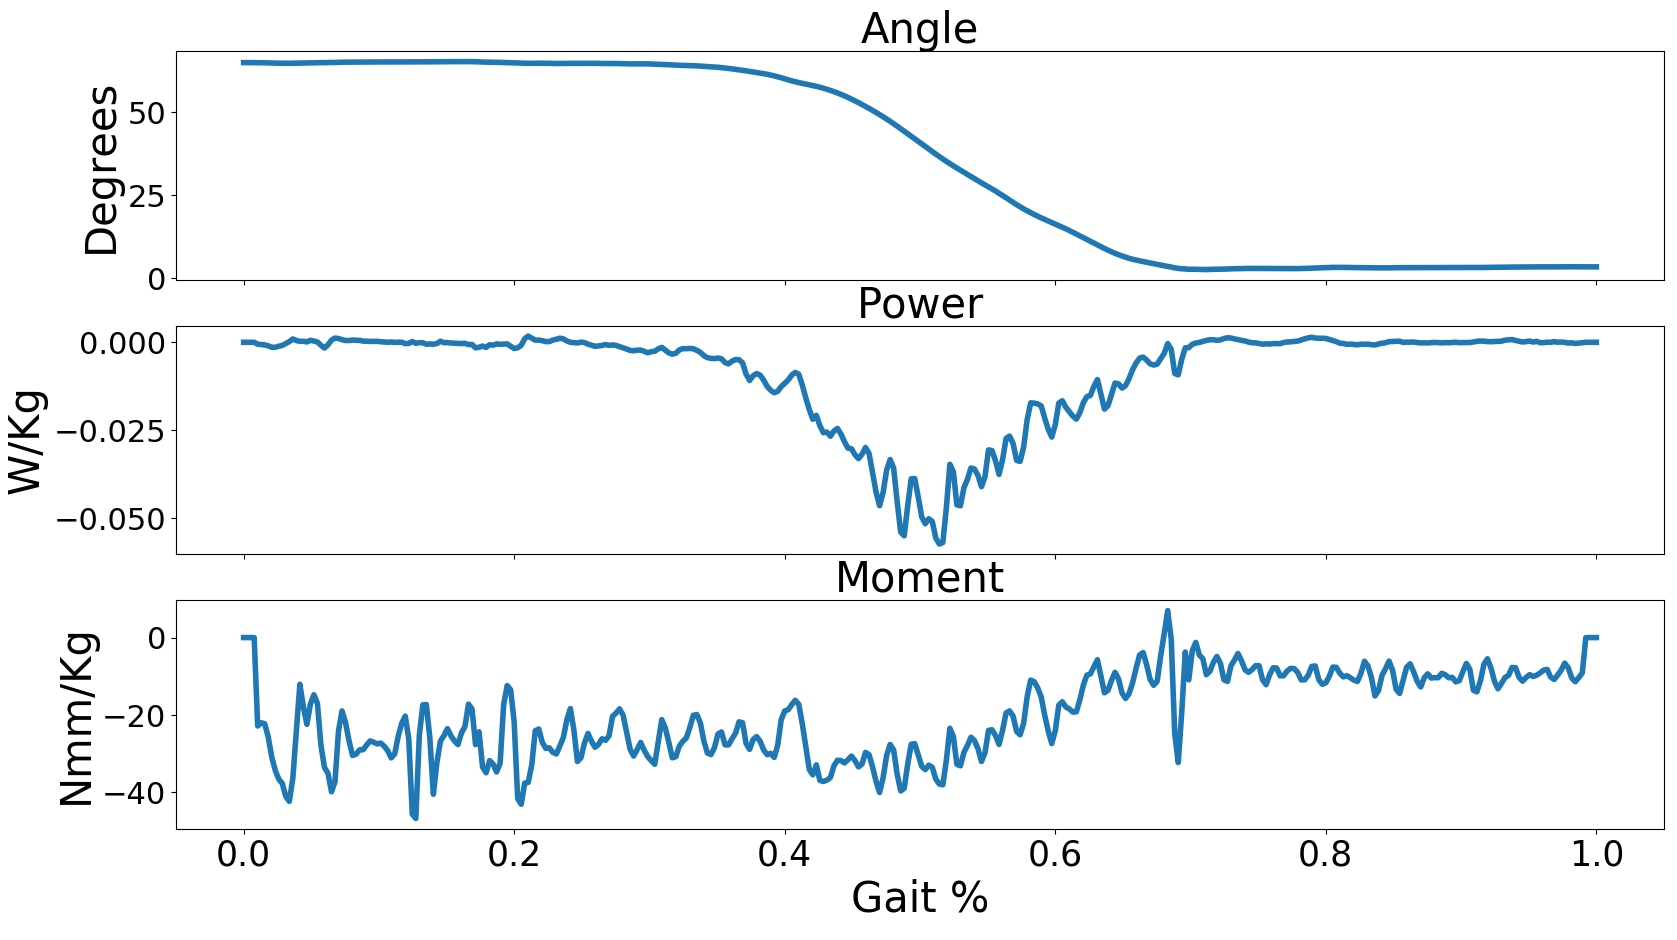
\includegraphics[width=\linewidth]{Figures/Design/SitStandPowerCurveKnee.png}
    \caption{Joint kinematics and dynamics during a sit/stand gait cycle \cite{SpringWrapClutchKnee}}
    \label{fig:SitStandPowerCurve}
\end{figure}

The knee joint has two rehabilitation requirements to fulfill: walking gaits and sit/stand gaits. Prior research has shown that walking gaits require roughly up to \(0.65 \frac{W}{kg}\) and \(0.25\frac{Nm}{kg}\), (see \autoref{fig:WalkingPowerCurve}), while a sit/stand gait requires roughly up to \(0.5 \frac{W}{kg}\) and \(0.04 \frac{Nm}{kg}\).  Speed requirements are roughly \(12^\circ/sec\) for walking gaits and \(15^\circ/sec\) for sit/stand gaits. Therefore, the designed knee joint for the \(100 kg\) weight specification should be capable of mechanically outputting \(65 W\) and \(25 Nm\) at \(15^\circ/sec\).

\subsubsection{Senses the joint angle}
Sensors must be able to accurately encode the rotational position of the joint. The rationale behind this requirement is for research, debugging, and most importantly accurate and safe position control. Therefore, the joint must be able to read its own position in both passive (non-powered) modes and active (powered) modes. It should also have a minimum accuracy of \(\pm0.5^\circ\) during position control, and be able to maintain position measurement through power cycles (absolute positioning).

\subsubsection{Simple to manufacture and assemble}
The joint must be designed with manufacturing and assembly in mind. All components must be easily sourced and generally available. Any machining requirement must be achievable with common machining techniques.

\subsubsection{Integrates into the WPI LARRE}
This research supports the advancement of the WPI LARRE project introduced in \autoref{sec:larre}. Therefore, the designed joint must be able to integrate into the universal exoskeleton joint connector developed in the LARRE project.

\section{Mechanical Design}

The orthotic joint design proposed uses a similar idea to how a human knee joint works; a cam mechanism  extends the shank link as it is rotated relative to the thigh link. The joint therefore has two degrees of freedom: rotation around the center of rotation (output shaft of the motor and gearbox) and translation in the direction of the shank. However, since there is only one actuator, the joint is underactuated; this underactuation can be taken advantage of to match a patient's knee trajectory, where the center of mass of the shank extends away from the joint center as the joint bends. For ease of assembly, the entire joint is held together by 4 M5 shoulder bolts, which also act as the axles for a total of 10 bearings. 

\begin{figure} [ht!]
    \centering
    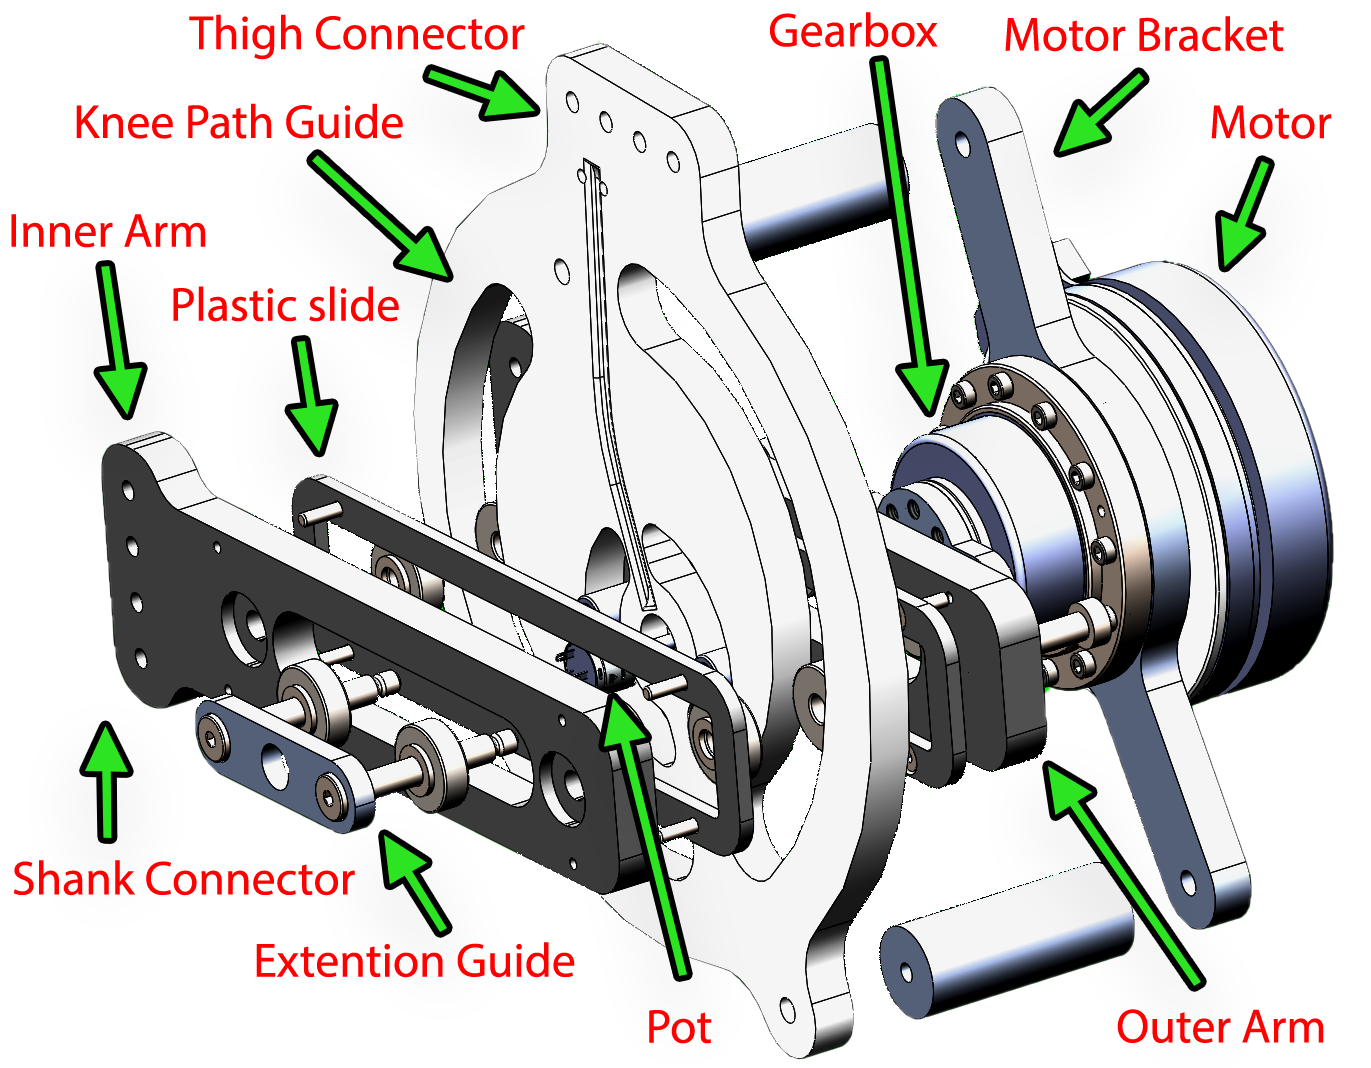
\includegraphics[width=0.8\linewidth]{Figures/Design/ExoKneeExplodedView.png}
    \caption{Exploded view of the knee joint, with all relevant components labeled}
    \label{fig:KneeJointExplodedView}
\end{figure}

\subsubsection{Torsion Bars}
The center of rotation of the joint is designed to match the axis of rotation of the actuator. The output of this actuator is directly connected to the torsion bar using M5 shoulder bolts. Each bolt is designed to support 3 bearings: 2 on the motor side and 1 on the patient side. The reduced count on the patient side allows for the torsion bar to be partially recessed in the shank link to reduce the distance between the center of mass between the patient and the joint. The 6 bearings are still able to support the forces necessary throughout a walking gait cycle (see \autoref{sec:BearingsAndCalcs}). 

\subsubsection{Shank Links}
The 2 shank links attach to the lower part of the exoskeleton, and are responsible for taking the rotational energy created by the motor and partially changing it to translational energy to help linearly extend the shank. The bearings connected to the torsion bars ride in a guide built into the shank link. This guide is slightly larger than the bearing diameter (\(~0.3mm\)) to prevent rubbing without creating much of a backlash (\(0.39^\circ\) backlash, see calculation on \autoref{eq:ShankLinkBacklash}).

\begin{equation}
    Backlash = atan(\frac{\frac{0.3mm}{2}}{22mm}) = 0.39^\circ
    \label{eq:ShankLinkBacklash}
\end{equation}

The surface of the guide must be smooth and parallel to the axis of the bearings to avoid damaging them. Depending on the material and manufacturing method chosen, the surface may require additional machining to ensure it can match these requirements. The length of the guide must be larger than the distance between the centers of the two shoulder bolts plus the maximum distance of linear extension by the knee (\autoref{eq:ExtensionGuideLength}). For this prototype, this length was \(78mm\).

\begin{equation}
    GuideLength \geq TorsionBarC2C + MaxKneeExtension = 44mm + 34mm = 78mm
    \label{eq:ExtensionGuideLength}
\end{equation}

The shank link is also responsible to connect to the lower part of the exoskeleton. Just like the thigh link, this is done through the universal exoskeleton connector developed throughout the WPI LARRE project \cite{SpringWrapClutchKnee}.

The connection between the thigh link and the shank link is very important, as it adds torsional stability and overall rigidness to the entire joint. It was therefore imperative during the design process to create wide surface contact between the thigh and shank links. To reduce the energy lost to friction between these plates, 3.2mm thick Delrin\textsuperscript{\textregistered} slides were laser cut and attached to the shank link. 

Similarly to the torsion bar, the shank link also uses 2 shoulder bolts to clamp the two shank links on the thigh link as well as to give the bearings that ride on the knee path guide a precise surface to mount to. To maintain a consistent clamping force, lock nuts are used since they do not easily back out with movement and vibration. 

\subsubsection{Thigh Link}

\begin{figure}[ht!]
    \centering
    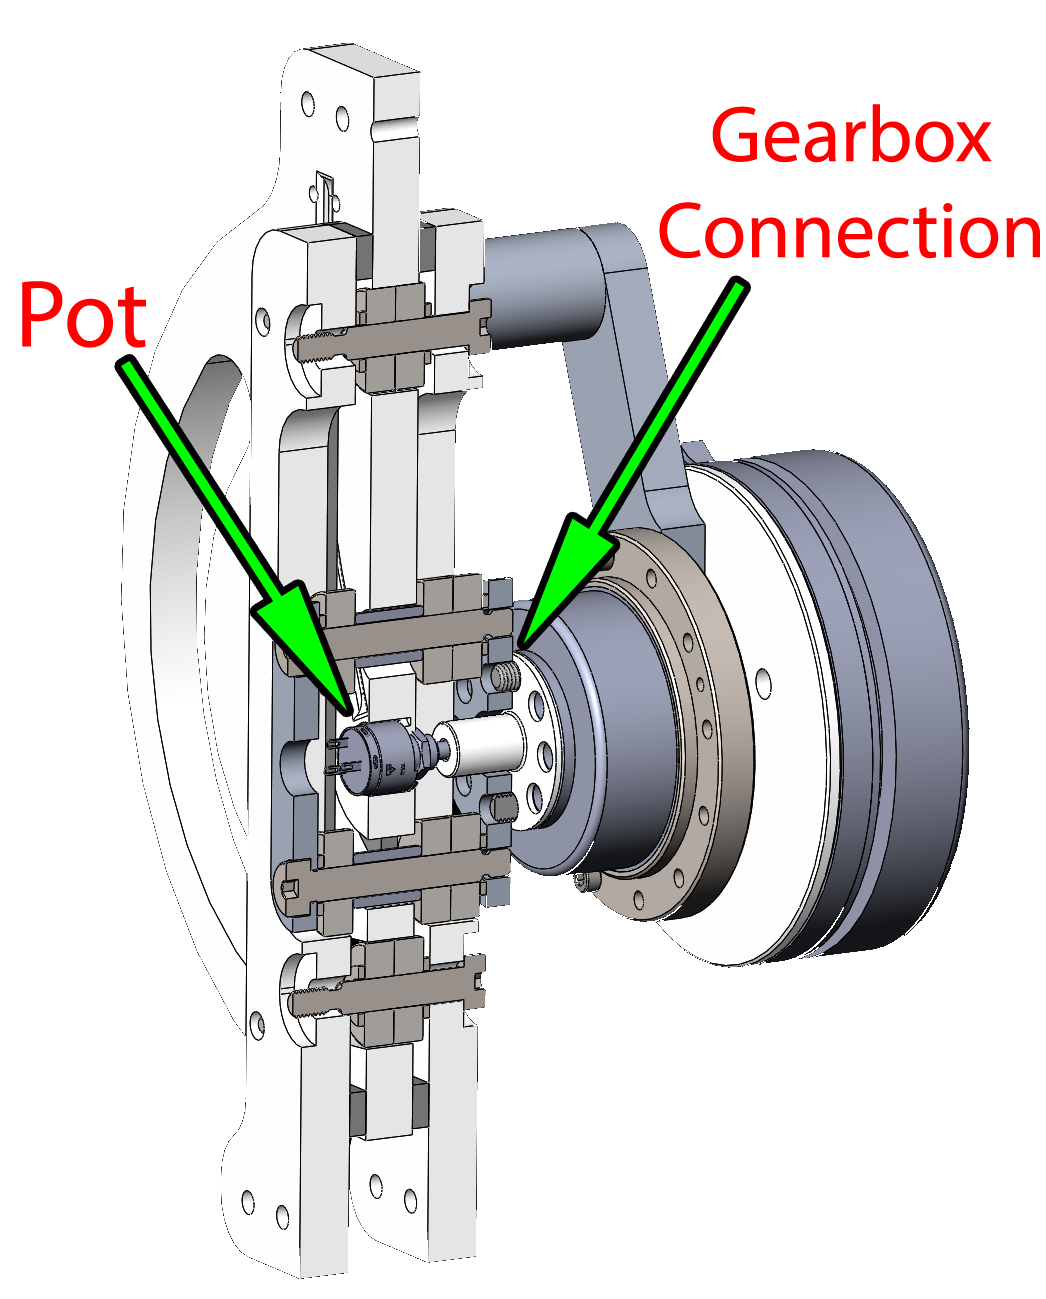
\includegraphics[width=0.7\linewidth]{Figures/Design/KneeJointAssyCrossSection_edit.png}
    \caption{A cross section of the knee joint in a \(0^\circ\) position}
    \label{fig:KneeJointCrossSection}
\end{figure}

The thigh link acts as the main mounting point for most things, as well as contains the knee path guide. Just like the shank link, the thigh link has the universal exoskeleton connector used throughout the WPI LARRE project. The motor bracket is connected to the thigh link at two locations using \(20mm\diameter x 50mm\) spacers. These spacers must be strong and stiff, as they transmit the torque between the thigh and shank connector in high load situations. A potentiometer is also mounted inside the thigh link to measure the current angle of the joint, as shown in \autoref{fig:KneeJointCrossSection}. The wire connecting to it is routed through a slot in the thigh link to avoid any interference with the moving shank links. This wire comes out the top and is connected to the main controller of the exoskeleton.

\subsubsection{Knee Path Guide}
The knee path guide is built into the thigh link as a slot. The geometry is calculated using several point measurements connected in SolidWorks with a spline. Each point is split by 15 degrees, and calculated from a pre-determined equation. This equation can be measured from a patient knee (see \autoref{sec:KneeParams}), but throughout the design and testing of this knee joint, \autoref{eq:KneeJointGeometryEquation} from \cite{KinDynKneeJoint} is used. \autoref{fig:CenterPlateGeometry} shows the equation above overlayed on the thigh link.

\begin{figure}[ht!]
    \centering
    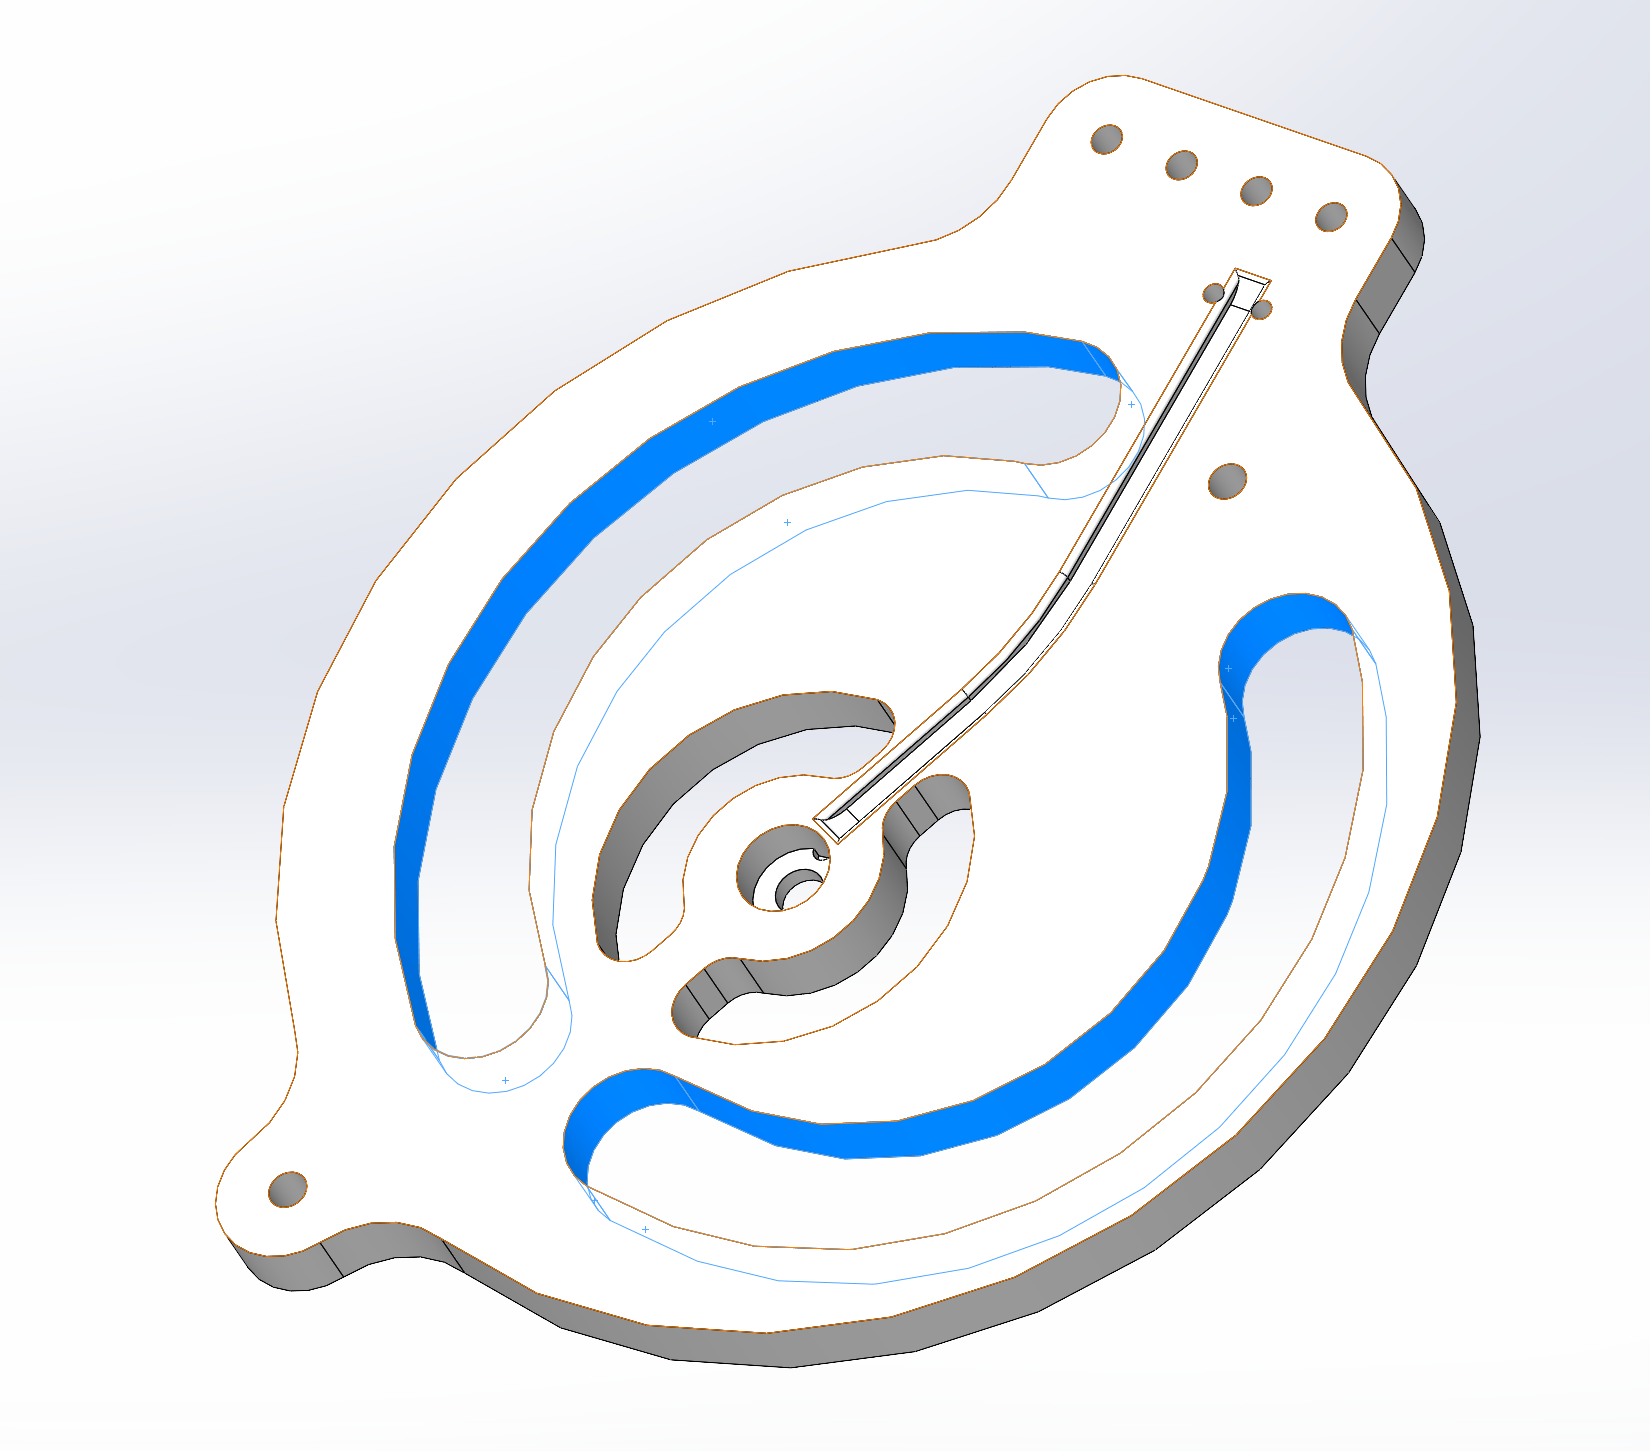
\includegraphics[width=0.8\linewidth]{Figures/Design/KneePathGuide.png}
    \caption{The thigh link contains the geometry (highlighted in blue) which the bearings ride on to mimic the tibiofemoral relationship}
    \label{fig:CenterPlateGeometry}
\end{figure}

The joint is designed to be easily adaptable between patients. Therefore, the only customized part in the entire system is the thigh link which holds the knee path guide. All other parts remain the same to decrease cost and improve repairability.

\subsubsection{Torque Requirements \& Actuator Selection}

The design parameters specified in \autoref{sec:DesignParams} are an output of at least \(65 W\) and \(25 Nm\) at \(15^\circ/sec\). The Maxon EC90 was chosen, with a peak power output of \(90W\) and a max continuous torque of \(0.560 Nm\) at \(2510 rpm\) (see \autoref{apx:EC90Datasheet}). To match the speed and torque requirements, a \(100:1\) gearbox ratio is needed. Due to its high reduction to size ratio, a strain wave gearbox from {Harmonic Drives\texttrademark} was chosen.\footnote{The gearbox used is proprietary, and no datasheet is available} Estimated efficiency of this gearbox is roughly \(\epsilon = 90\%\).

\begin{table}
    \centering
    \begin{tabular}{||c|c|c||}
        \hline
        Input (Motor) Power & \(P_{input}\) & \(90 Watts\) \\
        \hline
        Input (Motor) Torque @ Nominal & \(\tau_{input}\) & \(0.560 Nm\) \\
        \hline
        Input (Motor) Speed @ Nominal & \(\omega_{input}\) & \(2510 rpm\) \\
        \hline
        Input (Motor) Stall Torque & \(\tau_{in\_stall}\) & \(7.480 Nm\) \\
        \hline \hline
        Gearbox Ratio & \(\frac{n_1}{n_2}\) & \(100:1\) \\
        \hline \hline
        Output Power & \(P_{output}\) & \(81 Watts\) \\
        \hline
        Output Torque @ Nominal & \(\tau_{input}\) & \(50.4 Nm\) \\
        \hline
        Output Speed @ Nominal & \(\omega_{input}\) & \(15^\circ/sec\) \\
        \hline
        Output Stall Torque & \(\tau_{out\_stall}\) & \(673.2 Nm\) \\
        \hline
    \end{tabular}
    \caption{Motor/gearbox specifications and output power specifications of the proposed joint. See \autoref{apx:JointPowerTorqueSpeedCalcs} for all equations and calculations used.}
    \label{table:MotorGearboxSpecs}
\end{table}

The output power of the joint is \(81 W\), with a nominal torque of \(50.4 Nm\) at \(15^\circ/sec\). Power, torque, and speed specifications of the joint theoretically exceed the requirements. Physical testing is needed, however, to ensure that these numbers are accurate and sufficient for a rehabilitation exoskeleton.
 
\subsubsection{Potentiometer and Rotary Encoder}
A potentiometer was embedded into the knee design to act as an absolute rotary encoder to measure the current angle of the joint. It's purpose is twofold: to provide for an absolute angle at any given time and to provide for rough rotary encoding when a the motor (for passive experimentation). As mentioned above, the integration needed to protect the sensitive connection points. The potentiometer chosen was the Vishay PRV6, with \(200^\circ\) of travel, a linear resistance, and \(\pm 1\%\) tolerance, which equates to a sensored tolerance of \(\pm 2^\circ\). 

The motor used also has 3 hall sensors used for pinpointing the position of the rotor versus the stator. Since the motor has a 12 poles and 3 sensors (totaling 36 pulses per revolution) as well as a 100:1 reduction through the gearbox, the hall effect sensors can be used to create an effective 3600 pulses per revolution encoder. When used in conjunction with the absolute encoder, the encoded angle can be very precise.

% \subsubsection{Motor Analog} 
% \TODO{change the name of this}
% \TODO[inline]{Talk about motor/gearbox analog}

\subsubsection{Bearings}
\label{sec:BearingsAndCalcs}
All 10 bearings used in the design are the same (for simplicity and reduction of cost): 19mm outside diameter x 6mm inside diameter x 6mm thick double shielded ball bearings (Model 626ZZ). Each is rated for \(2.6kN\) dynamic load and \(1.05kN\) static load. Before selecting these bearings, two calculations were required to ensure these bearings could support the forces required.

The first is the requirement of the torsion bar. Given the max torque requirement for the project is \(25Nm\) and the torsion bar is \(44mm\) from center to center, \autoref{eq:TorsionBearingLoad} calculates that the total load on all 6 bearings used is \(1136N\), equaling to roughly \(190N\) per bearing.

\begin{equation}
    \text{Total Load per Torsion Bar Bearing}: \frac{1}{6} \times \frac{25Nm}{44mm / 2} = \frac{1}{6} \times \frac{25Nm}{0.022m} = 189.4N
    \label{eq:TorsionBearingLoad}
\end{equation}

The second force requirement for these bearings were in the knee path cam. Each knee joint must be able to hold half of the weight requirement of \(100kg\) statically. \autoref{eq:CamBearingLoad} demonstrates that each of the 4 bearings used in the cam will see a maximum static load of \(245N\) per bearing.

\begin{equation}
    \text{Total Load per Cam Bearing}: \frac{1}{4} \times 100kg \times 9.81m/s = 245.3N
    \label{eq:CamBearingLoad}
\end{equation}

% TODO: Probably should have a Design Analysis section, but not much data

\section{Material Selection \& Manufacturing}

The concept behind the joint is not dependent on material choice. However, when it came time to manufacture the prototypes, two materials were selected as potential options: aluminum and polylactic acid (PLA) plastic. Aluminum benefits from its strength to weight ratio and manufacturing simplicity when it is being machined. PLA plastic, on the other hand, can be injection molded or 3D printed using fused deposition modeling (FDM) printers. This makes PLA more flexible and less expensive, at the cost of softness and strength when compared to aluminum.

Other plastics and metals were initially considered. Out of the 3D printable plastics that were accessible with the tools available, PLA is strongest, stiffest, and hardest. Other FDM 3D printable plastics considered were  acrylonitrile butadiene styrene (ABS) and polyethylene terephthalate (PET). On the metals, side, steels were considered as a material option. However, its density and higher complexity to machine when compared to aluminum ruled it out as a material option.

\subsubsection{Material Analysis}
To decide between aluminum and PLA, the materials were analyzed in finite element analysis (FEA) simulation inside Dassault SolidWorks. \autoref{table:MaterialProperties} shows the material properties used. It is important to note that manufacturing methods were not considered in the analysis; therefore, layer adhesion was not considered when calculating the strength of the material.

\begin{table}
    \centering
    \begin{tabular}{ |c|c|c| }
        \hline
        Material & Aluminum & PLA \\
        \hline \hline
        Mass Density [$kg/m^3$] & 2700 & 1420 \\
        \hline
        Tensile Strength [$N/mm^2$] & 124.08 & 57.3\\
        \hline
        Yield Strength [$N/mm^2$] & 55.15 & 14.3\\ 
        \hline
        Shear Modulus [$N/mm^2$] & 26000 & 55000\\
        \hline
    \end{tabular}
    \caption{Material properties used when analyzing each material in FEA simulation in SolidWorks}
    \label{table:MaterialProperties}
\end{table}

\begin{figure}[ht!]
    \centering
    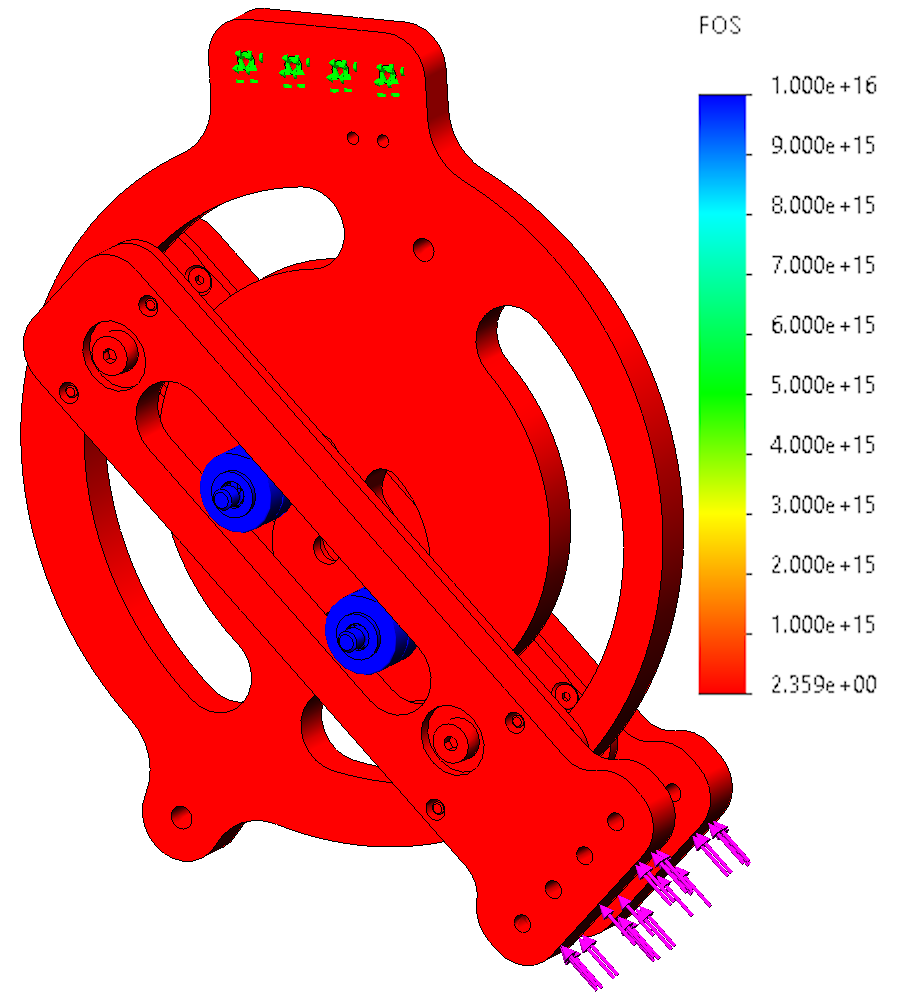
\includegraphics[width=0.8\linewidth]{Figures/Design/FEA_PLA_45deg.png}
    \caption{FEA of knee joint manufactured from PLA. Force applied (at arrows) is 500N, the resultant safety factor is 2.359.}
    \label{fig:FEA_PLA}
\end{figure}

\begin{figure}[ht!]
    \centering
    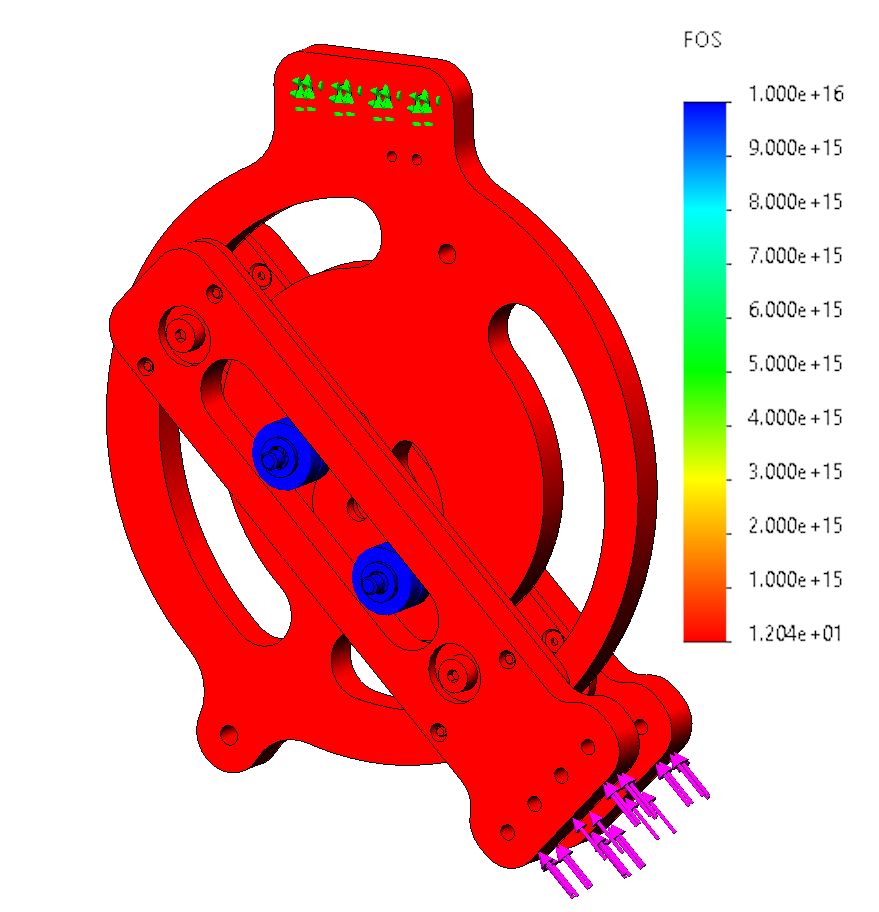
\includegraphics[width=0.8\linewidth]{Figures/Design/FEA_AL_45deg.png}
    \caption{FEA of knee joint manufactured from Aluminum. Force applied (at arrows) is 500N, the resultant safety factor is 12.04.}
    \label{fig:FEA_AL}
\end{figure}

PLA was chosen as the best material for our experimentation. Analysis demonstrated that it can support the stresses required at angle (shown in \autoref{fig:StrengthFlexion}). It can also be manufactured very quickly and easily with access to a conventional FDM 3D printer, allowing for quick revisions during the prototyping process. The final prototype was manufactured out of both aluminum and PLA; the thigh and shank links were 3D printed in PLA plastic while the torsion bar was machined out of aluminum to support the torque required.

However, if this joint were to be manufactured for use outside of prototype development and clinical trials, I would recommend using aluminum, as the joint would likely be more resilient and last longer. It would also increase torsional stiffness in the joint and reduce the likelihood of the bearings creating divots in the surface of the knee path guide.

\begin{figure}[ht!]
    \centering
    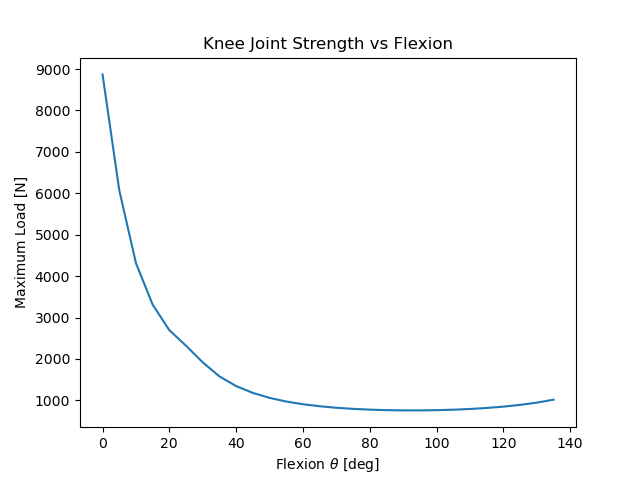
\includegraphics[width=0.8\linewidth]{Figures/Design/StrengthFlexionCurve.png}
    \caption{Analysis of the joint with major components manufactured out of PLA shows that the design is weakest at a \(90^\circ\) flexion, with a maximum static load of \(757N\) per joint.}
    \label{fig:StrengthFlexion}
\end{figure}

\subsubsection{Manufacturing}

The manufacturing process between the two materials is very different as well. While there are many different ways of creating parts in either material, the research will focus on the most common ways as to be easily replicated by others if desired.

As a plastic, PLA has many options for manufacturing. While PLA can be injection molded or machined, the most common use case for it is through FDM 3D printing. The accessibility and low cost at low production numbers makes this method of manufacturing the best for our use cases for the larger of our parts as well as any part that doesn't deal with big forces. For this project, a Creality Ender 3 was used to 3D print the parts required. 

Aluminum can also be 3D printed, but this requires some very specific tools to achieve. It can also be casted (similarly to injection molding for plastics), but this requires specific machining for the molds, and the parts still usually need to be machined to the final correct dimensions (the best option for high volume manufacturing). Therefore, all aluminum parts were designed to be manufactured using conventional lathes and mills. The manufacturing process, however, can be further simplified with access to a water jet or metal laser cutter. Such a tool can cut out all parts to a rough dimension, and a quick machining pass can finish the surfaces that need to be precise, such as the knee path guide and the slot in the shank link. If water jetting is selected as the preferred method of manufacture, parts may have a slight bevel due to the conical output of the water jet.

\section{Knee Trajectory Testing}
Motion capture and SolidWorks motion simulations were used to verify the joint's trajectory based on an inputted tibiofemoral trajectory. The motion simulation outputted a perfect match to the input equation (\autoref{eq:KneeJointGeometryEquation}), since the simulation platform is using a perfect model which directly inputs the equation above.

\begin{figure}[ht!]
    \centering
    \includegraphics[width=0.8\linewidth]{Figures/Design/KneeTrajTest.png}
    \caption{Experimental setup for measuring the trajectory of the manufactured joint. 9 motion capture dots were used to measure any movement in all 6 degrees of freedom.}
    \label{fig:TrajTestSetup}
\end{figure}

To further verify the relationship, a 10-camera Vicon Vantage 5 motion capture system was used. 9 motion capture dots were placed strategically around the knee joint. Two rigid bodies were used (each containing 4 motion capture dots) to be able to measure position and orientation in all 6 degrees of freedom. One rigid body was placed on the connector on the shank link, while the other was attached to the connector of the thigh link. A final motion capture dot was placed at the joint center. Then, the joint was manually actuated through its range while collecting data from the motion capture system. The data was processed using software tools developed in \autoref{sec:KneeParams} for measuring human tibiofemoral relationships. To ensure the data collected remained representative of the test and was not modified by any processing tools developed, only data importing tools were used. These tools simply took the raw data from the Vicon system and imported it into Python in a cleaner way.

\begin{figure}[ht!]
    \centering
    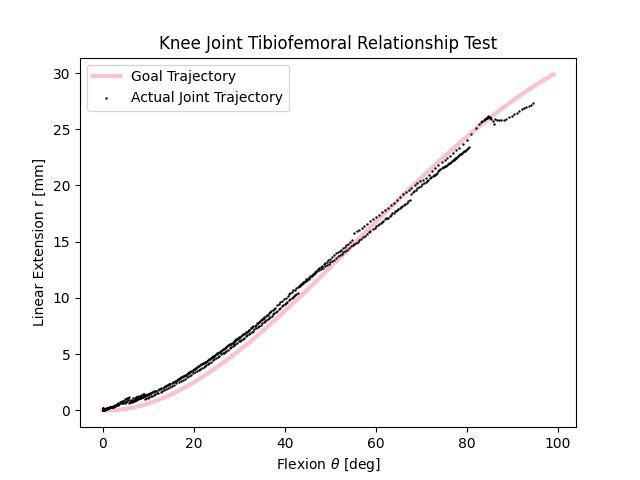
\includegraphics[width=0.8\linewidth]{Figures/Design/FlexionExtensionKneeJoint.png}
    \caption{Results from the motion capture system demonstrates that the designed knee joint can follow a desired trajectory very closely, only deviating by \(1mm\) maximum}
    \label{fig:TrajTestResults}
\end{figure}

The motion capture analysis data in \autoref{fig:TrajTestResults} demonstrates the effectiveness of the joint; it was able to follow the desired trajectory layed out in \autoref{eq:KneeJointGeometryEquation} with minimal error (deviation from goal trajectory under \(1mm\)). 